\subsubsubsection{non-native-inv}

\begin{enumerate}
    \item \verb|Target|: Check the modular inverse relation among three non-native target objects.
    \item \verb|Constraints logic|:
    \begin{itemize}
        \item Check equation for gadget: \verb|a * inv_a = 1 + modular * div|.
    \end{itemize}
    \item \verb|Process layout|: See \figref{fig:non-native-inv-layout}.
    \item \verb|Constraints info and costs|:
    \begin{itemize}
        \item gadget biguint-add num: 1
        \item gadget biguint-mul num: 2
        \item gate type num: 8 = 7 (U32AddManyGate\{3,5,7,9,11,13,15\}) + 1 (U32ArithmeticGate)
        \item gate instance num: 56 = (8 * 8 + 2) * 2 / 3 + 5 (U32AddManyGate{3}) + 5 + 2 (U32AddManyGate{15})
        \item copy-constraints: 762 = (8 * 8 + 2) * 2 * 3 + 21 * 4 + (6 + 8 + 10 + 12 + 14) * 4 + 4 * 16 + 18
    \end{itemize}
\end{enumerate}

\begin{figure}[!ht]
    \centering
    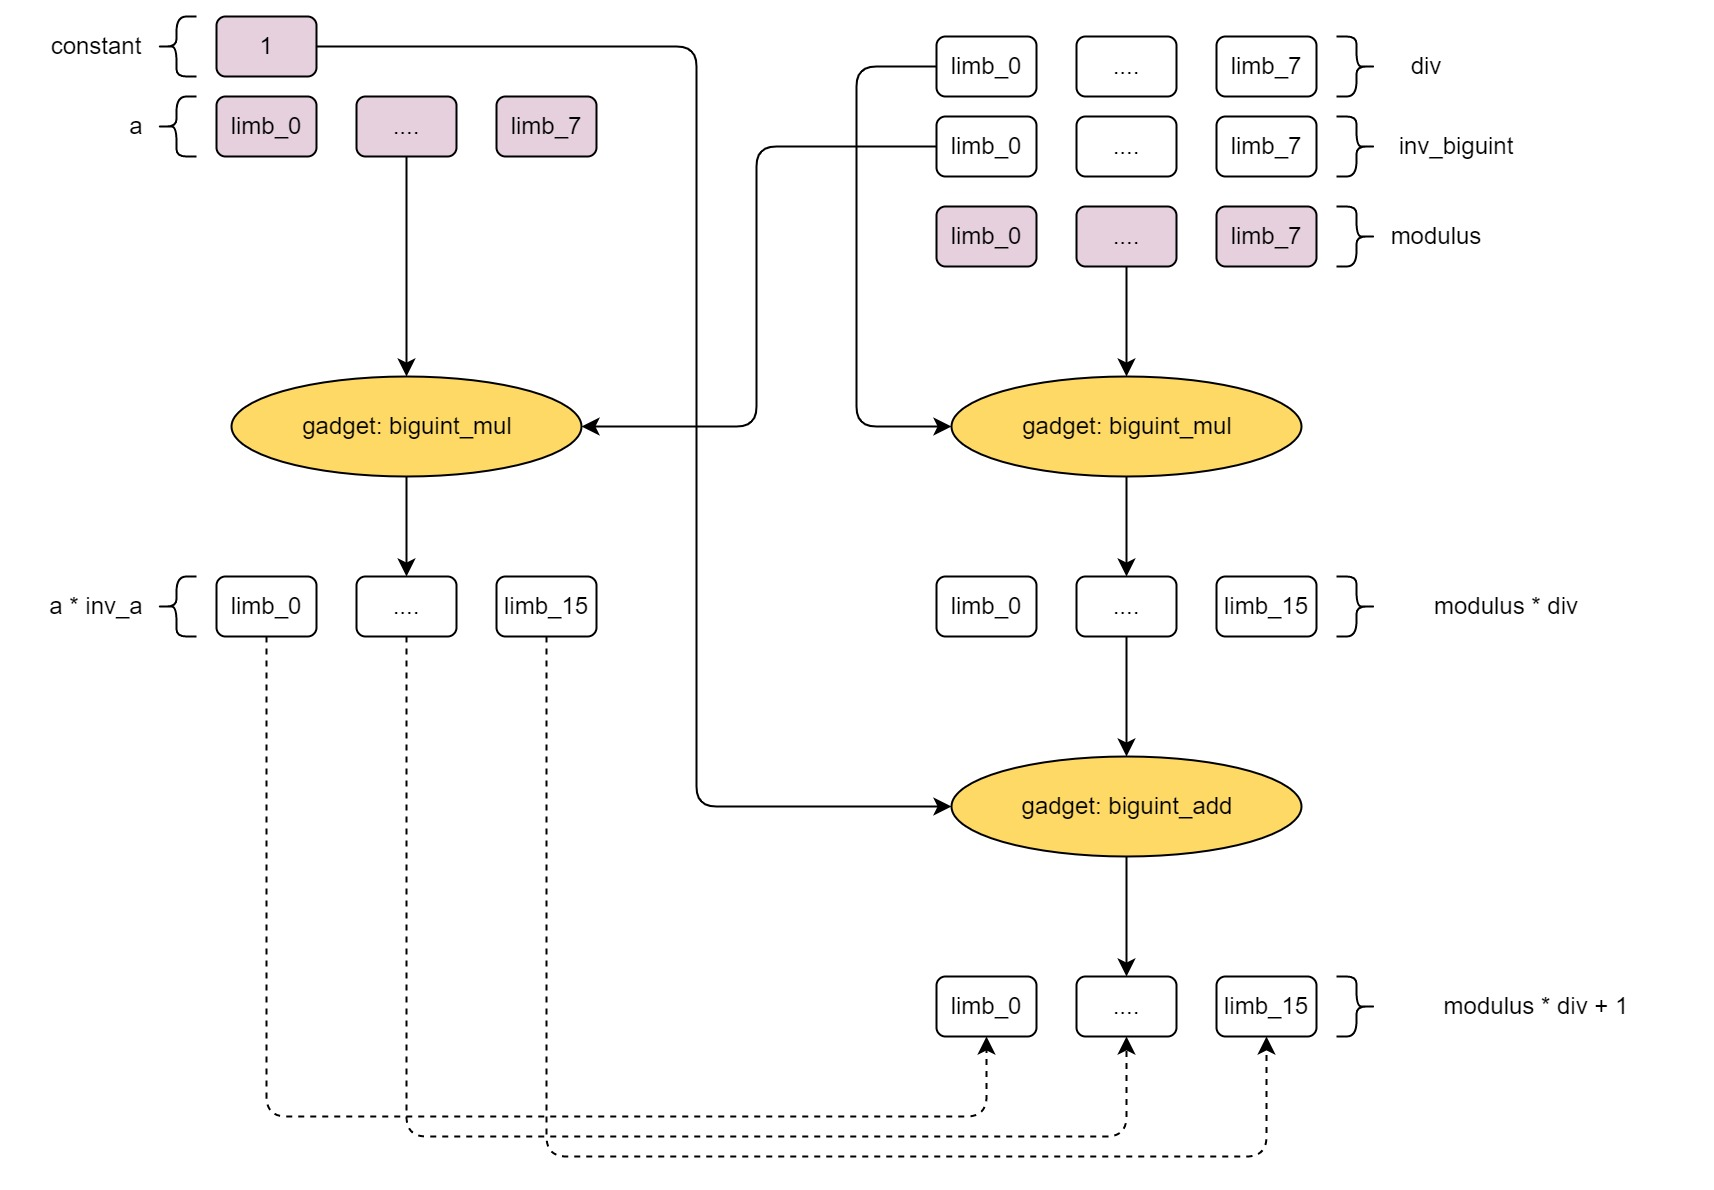
\includegraphics[width=0.6\textwidth]{nonnative-inv-layout.jpg}
    \caption{non-native-inv layout}
    \label{fig:non-native-inv-layout}
\end{figure}
